% !TEX root = paper.tex
% !TEX encoding = UTF-8 Unicode
% -*- coding: UTF-8; -*-
% vim: set fenc=utf-8
% !TEX spellcheck = en-US
\section{Results}
\label{sec:results}



%------------------------------%
%: see Figure~\ref{fig:results}
\begin{figure}%[!ht]%%[p!]
\centering{(A) \hspace{2.2cm} (B) \hspace{2cm} (C) \hspace{4.6cm} (D)\hspace{1.1cm}}
\centering{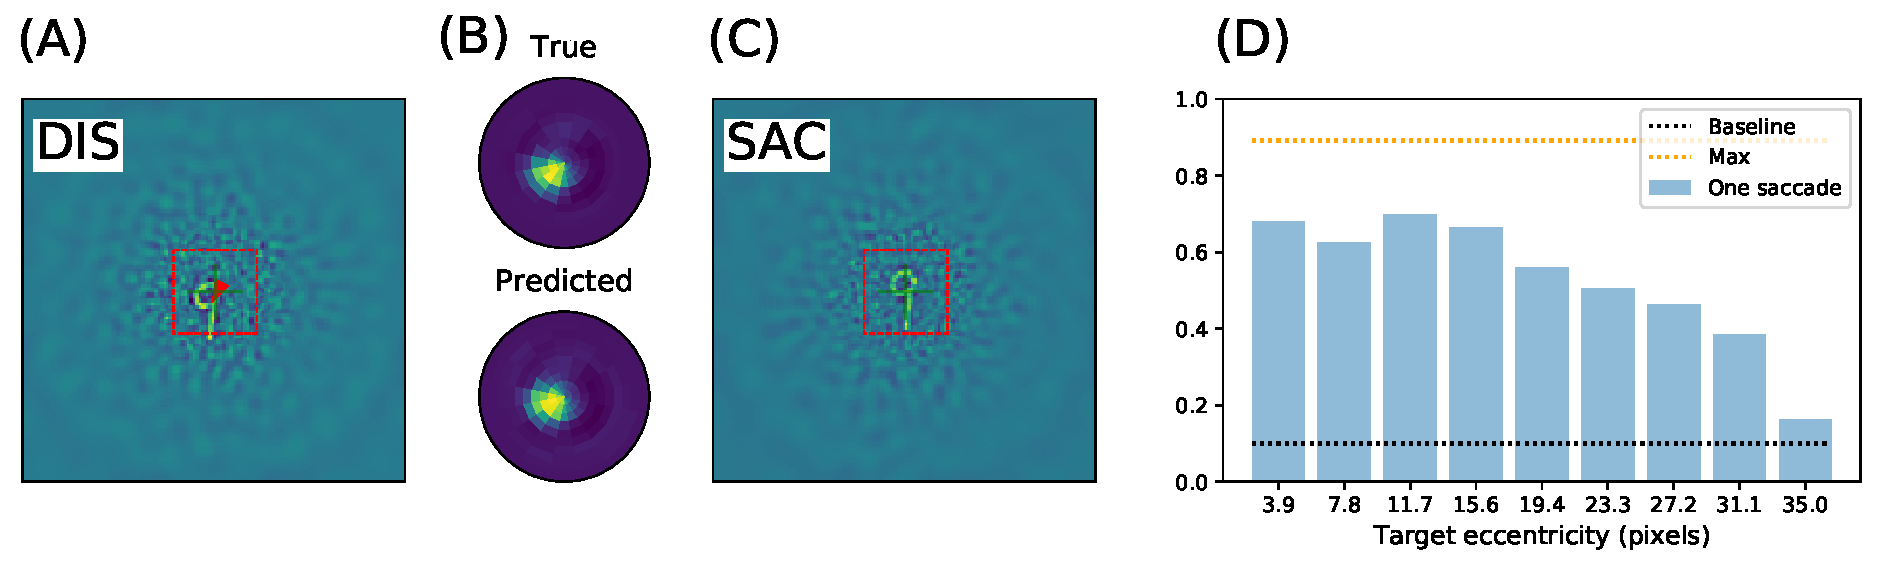
\includegraphics[width=\linewidth]{fig_result}}
\caption{
{\bf Simulated active vision agent}: 
(A)~The visual display ('DIS', see  Figure~\ref{fig:results}-C)  is transformed into a retinotopic representation which is used as the input of a multi-layer neural network, that transforms the retinal image into an accuracy map. (B)~After training, a typical network output  ('Predicted') is compared  with the ground truth ('True'). (C)~The network output allows to generate a saccade to the most likely target position in visual space, making possible to estimate a final classification rate. (D)~ Blue bars: Final classification rate after one saccade, in function of the target eccentricity, using the log-polar encoding scale (2, 3, 4.5, 6.5, 9, 13, 18, 26 and 36.5 pixels away from the center), averaged over 1,000 trials per eccentricity scale. Orange bars: accuracy of a central classifier, in function of the target eccentricity ('No saccade').
\label{fig:results}}%
\end{figure}%
%%------------------------------%
%result

After training the network, the categorical classifier accuracy is estimated as a function of the target initial eccentricity (see fig. \ref{fig:results}). For each different visual display (a different digit at a different position), a retinocentric visual input is processed (figure \ref{fig:results}A), providing a predicted accuracy map (figure \ref{fig:results}B) that can be compared to the actual future accuracy. Then a saccade is carried out based on the predicted accuracy map (figure \ref{fig:results}C), and the final accuracy is read from the 'True' accuracy map. This is repeated 1,000 times at different eccentricities, and the final average accuracy is shown on figure \ref{fig:results}D. It is compared to a central classifier trying to predict the category without doing a saccade.  
As expected, the  accuracy decreases with the eccentricity, for the targets become less and less visible in the periphery. 
The decrease is very rapid in the central classifier case: the accuracy drops to the baseline level after the third scale, which corresponds to a 6 pixels radius around the center of fixation). In contrast, issuing a saccade is beneficial in up to 8 spatial scales, which corresponds to a radius of about 26 pixels around the fixation center, allowing a much wider covering of the initial image. The difference between the two distributions forms an ``accuracy gain'', that quantifies the benefit of active inference with respect to a central prior, interpreted as the information gain provided by the ``Where'' pathway.

% energy consumption

% inhibition of return
As our saccade selection algorithm may implement the essential operations done in the ``Where'' pathway, the central classifier may also reflect the response of the ``What'' pathway,  
%A particular property of our agent is that at the time when the initial input is presented, two independent inferences are implemented. First, a
%The classification performed by the ``What'' pathway 
giving the potential identity of the digit. %Second, an accuracy map is predicted by the 'Where' pathway. 
It is therefore possible to compare the two accuracy estimates to chose the most appropriate action: it may be that the  accuracy is best in the ``What'' pathway and in that case no saccade is produced. 
The decision frontier lies between the first and the second spatial scale, allowing to pursue micro-saccades in the close vicinity of the target (2-3 pixels), in order to achieve a perfect centering.
In the other decision case, the ''What'' accuracy can still be considered to update the ``Where'' accuracy. 
%Indeed, one knows in particular the accuracy of the 'what' pathway when imposing small shifts to the input. 
This allows in particular to ``explain away" the current position of the fixation and the neighboring ones.
%(see line 'No saccade' in figure~\ref{fig:results}). 
Such heuristic gives a principled formulation of the inhibition of return mechanism which is an important aspect for modeling saccades~\citep{Itti01}. In particular, we predict that such a mechanism is dependent on the class of inputs, and would be different for searching for faces as compared to digits.
